\documentclass[10pt]{article}
\usepackage[utf8]{inputenc}
\usepackage[T1]{fontenc}
\usepackage{amsmath}
\usepackage{amsfonts}
\usepackage{amssymb}
\usepackage[version=4]{mhchem}
\usepackage{stmaryrd}
\usepackage{graphicx}
\usepackage[export]{adjustbox}
\graphicspath{ {./images/} }

\begin{document}
\section*{JEE-MAIN EXAMINATION - APRIL 2025}
(HELD ON WEDNESDAY \(\mathbf{2}^{\text {nd }}\) APRIL 2025)\\
TIME : 3:00 PM TO 6:00 PM

\section*{PHYSICS}
\section*{SECTION-A}
\begin{enumerate}
  \setcounter{enumi}{25}
  \item Given below are two statements: one is labelled as Assertion (A) and the other is labelled as Reason (R).\\
Assertion (A) : Net dipole moment of a polar linear isotropic dielectric substance is not zero even in the absence of an external electric field.
\end{enumerate}

Reason (R) : In absence of an external electric field, the different permanent dipoles of a polar dielectric substance are oriented in random directions.\\
In the light of the above statements, choose the most appropriate answer from the options given below :\\
(1) (A) is correct but (R) is not correct\\
(2) Both (A) and (R) are correct but (R) is not the correct explanation of (A)\\
(3) Both (A) and (R) are correct and (R) is the correct explanation of (A)\\
(4) (A) is not correct but (R) is correct

Ans. (4)\\
Sol. A : Since polar dielectrics are randomly oriental \(\overrightarrow{\mathrm{P}}_{\text {net }}=\overrightarrow{0}\).

R : If \(\overrightarrow{\mathrm{E}}\) is absent, polar dielectric remain polar \& are randomly oriented.\\
27. In a moving coil galvanometer, two moving coils \(\mathrm{M}_{1}\) and \(\mathrm{M}_{2}\) have the following particulars :\\
\(\mathrm{R}_{1}=5 \Omega, \mathrm{~N}_{1}=15, \mathrm{~A}_{1}=3.6 \times 10^{-3} \mathrm{~m}^{2}, \mathrm{~B}_{1}=0.25 \mathrm{~T}\)\\
\(\mathrm{R}_{2}=7 \Omega, \mathrm{~N}_{2}=21, \mathrm{~A}_{2}=1.8 \times 10^{-3} \mathrm{~m}^{2}, \mathrm{~B}_{2}=0.50 \mathrm{~T}\)\\
Assuming that torsional constant of the springs are same for both coils, what will be the ratio of voltage sensitivity of \(\mathrm{M}_{1}\) and \(\mathrm{M}_{2}\) ?\\
(1) \(1: 1\)\\
(2) \(1: 4\)\\
(3) \(1: 3\)\\
(4) \(1: 2\)

Ans. (1)\\
Sol. Voltage sensitivity \(=\frac{\theta}{\mathrm{V}}=\frac{\mathrm{NAB}}{\mathrm{cR}}\)\\
Ratio \(==\left(\frac{\mathrm{N}_{1} \mathrm{~A}_{1} \mathrm{~B}_{1}}{\mathrm{~N}_{2} \mathrm{~A}_{2} \mathrm{~B}_{2}}\right) \frac{\mathrm{R}_{2}}{\mathrm{R}_{1}}=\frac{15 \times 3.6 \times 0.25}{21 \times 1.8 \times 0.5} \times \frac{7}{5}=\frac{1}{1}\)

\section*{TEST PAPER WITH SOLUTION}
\begin{enumerate}
  \setcounter{enumi}{27}
  \item The moment of inertia of a circular ring of mass \(M\) and diameter \(r\) about a tangential axis lying in the plane of the ring is :\\
(1) \(\frac{1}{2} \mathrm{Mr}^{2}\)\\
(2) \(\frac{3}{8} \mathrm{Mr}^{2}\)\\
(3) \(\frac{3}{2} \mathrm{Mr}^{2}\)\\
(4) \(2 \mathrm{Mr}^{2}\)
\end{enumerate}

Ans. (2)\\
Sol. Diameter is given as R.\\
\(\therefore\) Radius \(=\mathrm{R} / 2\)\\
\(\mathrm{I}_{\text {tan gent }}=\frac{3}{2} \mathrm{~m}\left(\frac{\mathrm{R}}{2}\right)^{2}=\frac{3}{8} \mathrm{mR}^{2}\)\\
29. Two water drops each of radius ' \(r\) ' coalesce to from a bigger drop. If ' T ' is the surface tension, the surface energy released in this process is :\\
(1) \(4 \pi \mathrm{r}^{2} \mathrm{~T}\left[2-2^{\frac{2}{3}}\right]\)\\
(2) \(4 \pi \mathrm{r}^{2} \mathrm{~T}\left[2-2^{\frac{1}{3}}\right]\)\\
(3) \(4 \pi r^{2} T[1+\sqrt{2}]\)\\
(4) \(4 \pi \mathrm{r}^{2} \mathrm{~T}[\sqrt{2}-1]\)

Ans. (1)\\
Sol. \(\quad 2 \times \frac{4}{3} \pi R^{3}=\frac{4}{3} \pi r^{3} \Rightarrow r=2^{1 / 3} R\)\\
\(\mathrm{U}_{\mathrm{i}}=2 \times 4 \pi \mathrm{R}^{2} \mathrm{~T}\)\\
\(\mathrm{U}_{\mathrm{f}}=4 \pi \mathrm{r}^{2} \mathrm{~T}=4 \pi \mathrm{R}^{2} \mathrm{~T} 2^{2 / 3}\)\\
\(\therefore\) Heat lost \(=\mathrm{u}_{\mathrm{i}}-\mathrm{u}_{\mathrm{f}}=4 \pi \mathrm{R}^{2} \mathrm{~T}\left[2-2^{2 / 3}\right]\)\\
30. An electron with mass ' \(m\) ' with an initial velocity \((\mathrm{t}=0) \overrightarrow{\mathrm{v}}=\mathrm{v}_{0} \hat{\mathrm{i}}\left(\mathrm{v}_{0}>0\right)\) enters a magnetic field \(\overrightarrow{\mathrm{B}}=\mathrm{B}_{0} \hat{\mathrm{j}}\). If the initial de-Broglie wavelength at \(\mathrm{t}=0\) is \(\lambda_{0}\) then its value after time ' t ' would be :\\
(1) \(\frac{\lambda_{0}}{\sqrt{1-\frac{\mathrm{e}^{2} \mathrm{~B}_{0}^{2} \mathrm{t}^{2}}{\mathrm{~m}^{2}}}}\)\\
(2) \(\frac{\lambda_{0}}{\sqrt{1+\frac{\mathrm{e}^{2} \mathrm{~B}_{0}^{2} \mathrm{t}^{2}}{\mathrm{~m}^{2}}}}\)\\
(3) \(\lambda_{0} \sqrt{1+\frac{e^{2} B_{0}^{2} t^{2}}{m^{2}}}\)\\
(4) \(\lambda_{0}\)

Ans. (4)\\
Sol. Magnetic field does not work\\
\(\therefore\) Speed will not charge, so De-Broglie wavelength remains same.\\
31. A sinusoidal wave of wavelength 7.5 cm travels a distance of 1.2 cm along the \(x\)-direction in 0.3 sec . The crest P is at \(\mathrm{x}=0\) at \(\mathrm{t}=0 \mathrm{sec}\) and maximum displacement of the wave is 2 cm . Which equation correctly represents this wave ?\\
(1) \(y=2 \cos (0.83 x-3.35 t) c m\)\\
(2) \(\mathrm{y}=2 \sin (0.83 \mathrm{x}-3.5 \mathrm{t}) \mathrm{cm}\)\\
(3) \(y=2 \cos (3.35 x-0.83 t) \mathrm{cm}\)\\
(4) \(y=2 \cos (0.13 x-0.5 t) \mathrm{cm}\)

Ans. (1)\\
Sol. \(v=\frac{\text { dis } \tan c e}{\text { time }}\)\\
\(\mathrm{v}=\frac{12}{0.3}=4 \mathrm{~cm} / \mathrm{s}\)\\
\(\mathrm{k}=\frac{2 \pi}{\lambda}=\frac{2 \pi}{7.5}=\frac{4 \pi}{15}=0.83\)\\
\(\mathrm{v}=\frac{\omega}{\mathrm{k}} \Rightarrow \omega=\mathrm{vk}=4 \times \frac{4 \pi}{15}=3.35\)\\
So \(\mathrm{y}=\mathrm{A} \cos (\mathrm{kx}-\omega \mathrm{t})\)\\
32. Given a charge q , current I and permeability of vacuum \(\mu_{0}\). Which of the following quantity has the dimension of momentum ?\\
(1) \(\mathrm{qI} / \mu_{0}\)\\
(2) \(q \mu_{0} I\)\\
(3) \(q^{2} \mu_{0} I\)\\
(4) \(q \mu_{0} / I\)

Ans. (2)\\
Sol. \(\mathrm{Q}=\mathrm{AT}\)\\
\(\mathrm{I}=\mathrm{A}\)\\
\(\mu_{0}=\mathrm{MLT}^{-2} \mathrm{~A}^{-2}\)\\
\(\mathrm{P}=\mathrm{Q}^{\mathrm{x}} \mu_{0}{ }^{\mathrm{y}} \mathrm{I}^{\mathrm{z}}=[\mathrm{AT}]^{\mathrm{x}}\left[\mathrm{MLT}^{-2} \mathrm{~A}^{-2}\right]^{\mathrm{y}}[\mathrm{A}]^{\mathrm{z}}\)\\
\(\mathrm{MLT}^{-1}=\mathrm{M}^{\mathrm{y}} \mathrm{L}^{\mathrm{y}} \mathrm{T}^{\mathrm{x}-2 \mathrm{y}} \mathrm{A}^{-2 \mathrm{y}+\mathrm{z}+\mathrm{x}}\)\\
Now; \(\mathrm{y}=1\)\\
\(x-2 y=-1\)\\
\(-2 \mathrm{y}+\mathrm{z}=0\)\\
\(\therefore x=y=z=1\)\\
33. A solenoid having area A and length ' \(l\) ' is filled with a material having relative permeability 2 . The magnetic energy stored in the solenoid is :\\
(1) \(\frac{\mathrm{B}^{2} \mathrm{~A} l}{\mu_{0}}\)\\
(2) \(\frac{\mathrm{B}^{2} \mathrm{~A} l}{2 \mu_{0}}\)\\
(3) \(\mathrm{B}^{2} \mathrm{~A} l\)\\
(4) \(\frac{\mathrm{B}^{2} \mathrm{~A} l}{4 \mu_{0}}\)

Ans. (4)\\
Sol. \(\frac{U}{V}=\frac{B^{2}}{2 \mu_{r} u_{0}} \Rightarrow U=\frac{B^{2}}{4 \mu_{0}} V=\frac{B^{2}}{4 \mu_{0}} A \ell\)\\
34. Two large plane parallel conducting plates are kept 10 cm apart as shown in figure. The potential difference between them is V . The potential difference between the points A and B (shown in the figure) is :\\
\includegraphics[max width=\textwidth, center]{2025_10_05_e8cde6f242323cc9c307g-2(1)}\\
(1) \(\frac{1}{4} \mathrm{~V}\)\\
(2) \(\frac{2}{5} \mathrm{~V}\)\\
(3) \(\frac{3}{4} \mathrm{~V}\)\\
(4) 1 V

Ans. (2)\\
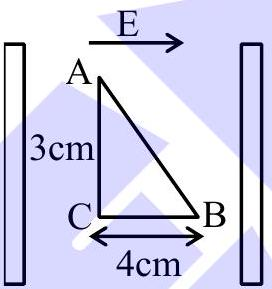
\includegraphics[max width=\textwidth, center]{2025_10_05_e8cde6f242323cc9c307g-2}

Sol.

\[
\begin{aligned}
& \text { Using } \Delta V=E(\Delta d) \\
& V=E(10) \\
& V_{A B}=E .4=\frac{V}{10} \times 4=\frac{2 V}{5}
\end{aligned}
\]

\begin{enumerate}
  \setcounter{enumi}{34}
  \item Identify the characteristics of an adiabatic process in a monoatomic gas.\\
(A) Internal energy is constant.\\
(B) Work done in the process is equal to the charge in internal energy.\\
(C) The product of temperature and volume is a constant.\\
(D) The product of pressure and volume is a constant.\\
(E) The work done to change the temperature from \(\mathrm{T}_{1}\) to \(\mathrm{T}_{2}\) is proportional to \(\left(\mathrm{T}_{2}-\mathrm{T}_{1}\right)\)\\
Choose the correct answer from the options given below :\\
(1) (A), (C), (D) only\\
(2) (A), (C), (E) only\\
(3) (B), (E) only\\
(4) (B), (D) only
\end{enumerate}

Ans. (3)\\
Sol. \(\mathrm{Q}=\Delta \mathrm{U}+\mathrm{W}=0 \Rightarrow-\Delta \mathrm{U}=\mathrm{W}\)

\[
\mathrm{WD}=-\mathrm{nC}_{\mathrm{v}} \Delta \mathrm{~T} \Rightarrow|\mathrm{WD}|=\mathrm{nC}_{\mathrm{v}} \Delta \mathrm{~T} \propto \mathrm{~T}_{2}-\mathrm{T}_{1}
\]

\(\therefore \mathrm{B} \& \mathrm{E}[\) Only possibility]\\
36. Assuming the validity of Bohr's atomic model for hydrogen like ions the radius of \(\mathrm{Li}^{++}\)ion in its ground state is given by \(\frac{1}{X} a_{0}\), where \(X=\) \(\_\_\_\_\) .\\
(Where \(\mathrm{a}_{0}\) is the first Bohr's radius.)\\
(1) 2\\
(2) 1\\
(3) 3\\
(4) 9

Ans. (3)\\
Sol. \(\quad r=r_{0} \frac{n^{2}}{z} \& z=3\) for \(L^{+2}\) and \(n=1\)\\
\(\therefore \mathrm{r}=\mathrm{r}_{0} \frac{1^{2}}{3}=\frac{\mathrm{r}_{0}}{3}\)\\
\(\therefore \mathrm{x}=3\)\\
37. Energy released when two deuterons \(\left({ }_{1} \mathrm{H}^{2}\right)\) fuse to form a helium nucleus \(\left({ }_{2} \mathrm{He}^{4}\right)\) is :\\
(Given : Binding energy per nucleon of \({ }_{1} \mathrm{H}^{2}=1.1 \mathrm{MeV}\) and binding energy per nucleon of \({ }_{2} \mathrm{He}^{4}=7.0 \mathrm{MeV}\) )\\
(1) 8.1 MeV\\
(2) 5.9 MeV\\
(3) 23.6 MeV\\
(4) 26.8 MeV

Ans. (3)\\
Sol. \(\underset{1.1 \mathrm{MeV}}{\mathrm{H}^{2}}+{ }_{1} \mathrm{H}^{2} \rightarrow \underset{7.0 \mathrm{MeV}}{\mathrm{He}^{4}}\)\\
\(\mathrm{E}_{\mathrm{B}}=\mathrm{BE}_{\text {reactant }}-\mathrm{BE}_{\text {product }}\)\\
\(=1.1 \times 2+1.1 \times 2-7 \times 4=-23.6 \mathrm{MeV}\)\\
\(=\mathrm{Q}=23.6 \mathrm{MeV}\)\\
38. In the digital circuit shown in the figure, for the given inputs the P and Q values are :\\
\includegraphics[max width=\textwidth, center]{2025_10_05_e8cde6f242323cc9c307g-3(2)}\\
(1) \(\mathrm{P}=1, \mathrm{Q}=1\)\\
(2) \(P=0, Q=0\)\\
(3) \(\mathrm{P}=0, \mathrm{Q}=1\)\\
(4) \(\mathrm{P}=1, \mathrm{Q}=0\)

Ans. (2)

Sol.\\
\includegraphics[max width=\textwidth, center]{2025_10_05_e8cde6f242323cc9c307g-3(4)}\\
39. Two identical objects are placed in front of convex mirror and concave mirror having same radii of curvature of 12 cm , at same distance of 18 cm from the respective mirrors. The ratio of sizes of the images formed by convex mirror and by concave mirror is :\\
(1) \(1 / 2\)\\
(2) 2\\
(3) 3\\
(4) \(1 / 3\)

Ans. (1)

Sol.\\
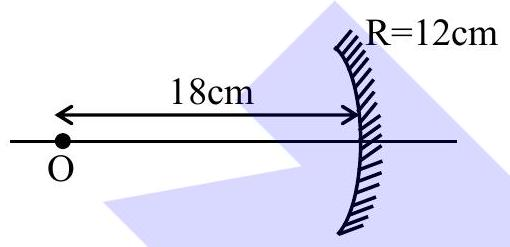
\includegraphics[max width=\textwidth, center]{2025_10_05_e8cde6f242323cc9c307g-3}

Using \(m=\frac{f}{u-f}\)\\
\(m_{1}=\frac{6}{18-6}=\frac{1}{2}\)\\
\includegraphics[max width=\textwidth, center]{2025_10_05_e8cde6f242323cc9c307g-3(3)}\\
40. A sportsman runs around a circular track of radius \(r\) such that he traverses the path \(A B A B\). The distance travelled and displacement, respectively, are\\
\includegraphics[max width=\textwidth, center]{2025_10_05_e8cde6f242323cc9c307g-3(1)}\\
(1) \(2 \mathrm{r}, 3 \pi \mathrm{r}\)\\
(2) \(3 \pi r, \pi r\)\\
(3) \(\pi r, 3 r\)\\
(4) \(3 \pi r, 2 r\)

Ans. (4)\\
Sol. Displacement \(=2 \mathrm{r}\)\\
Distance \(=2 \pi \mathrm{r}+\pi \mathrm{r}=3 \pi \mathrm{r}\)\\
41.\\
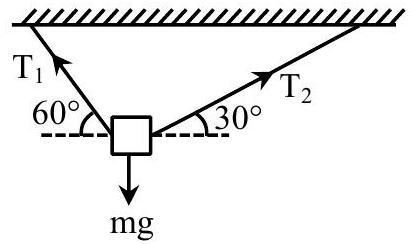
\includegraphics[max width=\textwidth, center]{2025_10_05_e8cde6f242323cc9c307g-4}

A body of mass 1 kg is suspended with the help of two strings making angles as shown in figure. Magnitude of tensions \(\mathrm{T}_{1}\) and \(\mathrm{T}_{2}\), respectively, are (in N) :\\
(1) \(5,5 \sqrt{3}\)\\
(2) \(5 \sqrt{3}, 5\)\\
(3) \(5 \sqrt{3}, 5 \sqrt{3}\)\\
(4) 5,5

Ans. (2)\\
\includegraphics[max width=\textwidth, center]{2025_10_05_e8cde6f242323cc9c307g-4(1)}

Sol.

\[
\begin{aligned}
& \mathrm{T}_{1}=\mathrm{mg} \cos 30^{\circ} \\
& \mathrm{T}_{2}=\mathrm{mg} \sin 30^{\circ}
\end{aligned}
\]

\begin{enumerate}
  \setcounter{enumi}{41}
  \item A bi-convex lens has radius of curvature of both the surfaces same as \(1 / 6 \mathrm{~cm}\). If this lens is required to be replaced by another convex lens having different radii of curvatures on both sides ( \(\mathrm{R}_{1} \neq \mathrm{R}_{2}\) ), without any change in lens power then possible combination of \(\mathrm{R}_{1}\) and \(\mathrm{R}_{2}\) is :\\
(1) \(\frac{1}{3} \mathrm{~cm}\) and \(\frac{1}{3} \mathrm{~cm}\)\\
(2) \(\frac{1}{5} \mathrm{~cm}\) and \(\frac{1}{7} \mathrm{~cm}\)\\
(3) \(\frac{1}{3} \mathrm{~cm}\) and \(\frac{1}{7} \mathrm{~cm}\)\\
(4) \(\frac{1}{6} \mathrm{~cm}\) and \(\frac{1}{9} \mathrm{~cm}\)
\end{enumerate}

Ans. (2)\\
Sol. This will happen when\\
\(\frac{1}{\mathrm{f}_{1}}=\frac{1}{\mathrm{f}_{2}}\)\\
\((\mu-1)\left(\frac{1}{\mathrm{R}_{1}}-\frac{1}{-\mathrm{R}_{2}}\right)=(\mu-1)\left(\frac{2}{\mathrm{R}}\right)\)\\
\(\frac{1}{\mathrm{R}_{1}}+\frac{1}{\mathrm{R}_{2}}=\frac{2}{\mathrm{R}}\)\\
43. If \(\mu_{0}\) and \(\varepsilon_{0}\) are the permeability and permittivity of free space, respectively, then the dimension of \(\left(\frac{1}{\mu_{0} \varepsilon_{0}}\right)\) is :\\
(1) \(\mathrm{L} / \mathrm{T}^{2}\)\\
(2) \(\mathrm{L}^{2} / \mathrm{T}^{2}\)\\
(3) \(T^{2} / L\)\\
(4) \(T^{2} / L^{2}\)

Ans. (2)\\
Sol. \(\mathrm{C}=\frac{1}{\sqrt{\mu_{0} \varepsilon_{0}}} \Rightarrow \frac{1}{\mu_{0} \varepsilon_{0}}=\mathrm{C}^{2}=\mathrm{L}^{2} \mathrm{~T}^{-2}\)\\
44. Match List-I with List-II.

\begin{center}
\begin{tabular}{ll}
\multicolumn{1}{c}{List-I} & \multicolumn{1}{c}{List-II} \\
(A) Heat capacity of body & (I) \(\mathrm{J} \mathrm{kg}^{-1}\) \\
(B) Specific heat capacity of body & (II) \(\mathrm{JK}^{-1}\) \\
(C) Latent heat & (III) \(\mathrm{J} \mathrm{kg}^{-1} \mathrm{~K}^{-1}\) \\
(D) Thermal conductivity & (IV) \(\mathrm{Jm}^{-1} \mathrm{~K}^{-1} \mathrm{~s}^{-1}\) \\
\end{tabular}
\end{center}

Choose the correct answer from the options given below:\\
(1) (A)-(III), (B)-(I), (C)-(II), (D)-(IV)\\
(2) (A)-(IV), (B)-(III), (C)-(II), (D)-(I)\\
(3) (A)-(III), (B)-(IV), (C)-(I), (D)-(II)\\
(4) (A)-(II), (B)-(III), (C)-(I), (D)-(IV)

Ans. (4)\\
Sol. \(\mathrm{C}^{\prime}=\frac{\Delta \mathrm{Q}}{\Delta \mathrm{T}}=\mathrm{JK}^{-1}\)\\
\(\mathrm{S}=\frac{\Delta \mathrm{Q}}{\mathrm{m} \Delta \mathrm{T}}=\mathrm{Jkg}^{-1} \mathrm{~K}^{-1}\)\\
\(\mathrm{L}=\frac{\Delta \mathrm{Q}}{\mathrm{m}}=\mathrm{Jkg}^{-1}\)\\
\(\Delta \mathrm{Q}=\frac{\mathrm{KA} \Delta \mathrm{T}}{\mathrm{L}} \Rightarrow \mathrm{K}=\frac{\Delta \mathrm{Q}(\mathrm{L})}{\mathrm{A} \Delta \mathrm{T}}=\mathrm{Jm}^{-1} \mathrm{~K}^{-1} \mathrm{~s}^{-1}\)\\
45. Consider a circular loop that is uniformly charged and has a radius \(\mathrm{a} \sqrt{2}\). Find the position along the positive \(z\)-axis of the cartesian coordinate system where the electric field is maximum if the ring was assumed to be placed in xy-plane at the origin :\\
(1) \(\frac{a}{\sqrt{2}}\)\\
(2) \(\frac{a}{2}\)\\
(3) a\\
(4) 0

Ans. (3)\\
Sol. \(\mathrm{E}=\frac{\mathrm{KQr}}{\left(\mathrm{x}^{2}+\mathrm{R}^{2}\right)^{3 / 2}}\)\\
\(\frac{\mathrm{dE}}{\mathrm{dx}}=0\)\\
\(\therefore x=\frac{R}{\sqrt{2}}=\frac{\sqrt{2} a}{\sqrt{2}}=a\)

\section*{SECTION-B}
46.

\begin{center}
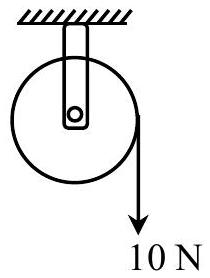
\includegraphics[max width=\textwidth]{2025_10_05_e8cde6f242323cc9c307g-5}
\end{center}

A wheel of radius 0.2 m rotates freely about its center when a string that is wrapped over its rim is pulled by force of 10 N as shown in figure. The established torque produces an angular acceleration of \(2 \mathrm{rad} / \mathrm{s}^{2}\). Moment of inertia of the wheel is \(\_\_\_\_\) \(\mathrm{kg} \mathrm{m}^{2}\).\\
(Acceleration due to gravity \(=10 \mathrm{~m} / \mathrm{s}^{2}\) )\\
Ans. (1)\\
\includegraphics[max width=\textwidth, center]{2025_10_05_e8cde6f242323cc9c307g-5(1)}

Sol.

\[
\begin{aligned}
& \mathrm{FR}=\mathrm{I} \alpha \\
& \Rightarrow \mathrm{I}=\frac{\mathrm{FR}}{\alpha}=\frac{10 \times 0.2}{2}=1 \mathrm{~kg}-\mathrm{m}^{2}
\end{aligned}
\]

\begin{enumerate}
  \setcounter{enumi}{46}
  \item The internal energy of air in \(4 \mathrm{~m} \times 4 \mathrm{~m} \times 3 \mathrm{~m}\) sized room at 1 atmospheric pressure will be \(\_\_\_\_\) \(\times 10^{6} \mathrm{~J}\).\\
(Consider air as diatomic molecule)\\
Ans. (12)\\
Sol.\\
To find the internal energy of gas in the room.\\
\(\mathrm{U}=\mathrm{nC}_{\mathrm{v}} \mathrm{T}=\mathrm{n} \frac{5 \mathrm{RT}}{2}\)\\
\(=\frac{5}{2} \mathrm{PV}=\frac{5}{2} \times 10^{5} \times 48=12 \times 10^{6} \mathrm{~J}\)
  \item A ray of light suffers minimum deviation when incident on a prism having angle of the prism equal to \(60^{\circ}\). The refractive index of the prism material is \(\sqrt{2}\). The angle of incidence (in degrees) is \(\_\_\_\_\) .
\end{enumerate}

Ans. (45)\\
Sol. \(\mu=\frac{\sin \left(\frac{A+\delta_{m}}{2}\right)}{\sin \left(\frac{A}{2}\right)}\), since \(A=60^{\circ} \quad \therefore \delta m=30^{\circ}\)\\
\(\delta_{\mathrm{m}}=2 \mathrm{i}-\mathrm{A}\) [as \(\mathrm{i}=\mathrm{e}\) ]\\
\(\Rightarrow \mathrm{i}=45^{\circ}\)\\
49. The length of a light string is 1.4 m when the tension on it is 5 N . If the tension increases to 7 N , the length of the string is 1.56 m . The original length of the string is \(\_\_\_\_\) m.

Ans. (1)\\
Sol. \(\mathrm{T}=\mathrm{K}\left(\ell-\ell_{0}\right)\)\\
\(\Rightarrow 5=\mathrm{K}\left(1.4-\ell_{0}\right)\)\\
\(\Rightarrow 7=\mathrm{K}\left(1.56-\ell_{0}\right)\)\\
\(\Rightarrow \frac{5}{1.4-\ell_{0}}=\frac{7}{1.56-\ell_{0}}\)\\
\(\therefore \ell_{0}=1 \mathrm{~m}\)\\
50. A satellite of mass 1000 kg is launched to revolve around the earth in an orbit at a height of 270 km from the earth's surface. Kinetic energy of the satellite in this orbit is \(\_\_\_\_\) \(\times 10^{10} \mathrm{~J}\).\\
(Mass of earth \(=6 \times 10^{24} \mathrm{~kg}\), Radius of earth \(= 6.4 \times 10^{6} \mathrm{~m}\), Gravitational constant \(= 6.67 \times 10^{-11} \mathrm{Nm}^{2} \mathrm{~kg}^{-2}\) )

Ans. (3)\\
Sol. \(\mathrm{KE}=\frac{1}{2} \mathrm{mv}^{2}=\frac{1}{2} \mathrm{~m} \frac{\mathrm{GM}_{\mathrm{e}}}{\mathrm{r}}=\frac{\mathrm{GM}_{\mathrm{e}} \mathrm{m}}{2 \mathrm{r}}=\frac{\mathrm{GM}_{\mathrm{e}} \mathrm{m}}{2\left(\mathrm{R}_{\mathrm{E}}+\mathrm{h}\right)}\)

\[
=\frac{6.67 \times 10^{-11} \times 6 \times 10^{24} \times 6.4 \times 10^{6}}{2\left(6.4 \times 10^{6}+2.7 \times 10^{5}\right)}=3 \times 10^{10} \mathrm{~J}
\]

\section*{Level up your prep for JEE with our LIVE JEE Courses!}
LIVE classes with top Kota faculty\\
ALLEN's study material\\
Tests with national benchmarking\\
ALLEN App Advantage: 24/7 doubt support, Custom Practice \& more

Enrol Now

\section*{ALLEN ONLINE}
\section*{Secure up to}
\section*{90\% scholarship on our Online Courses!}
\section*{based on your JEE Main 2025 scores!}
Enrol Now


\end{document}